\documentclass{report}
\usepackage{pdfpages}
\usepackage[a4paper, top=2cm, bottom=2cm, left=2cm, right=2cm]{geometry}
\usepackage{fancyhdr}
\usepackage{graphicx} 
\usepackage{ulem}
\usepackage{listings}
\usepackage[absolute,overlay]{textpos}
\usepackage{minted}

\lstdefinestyle{cppstyle}{
	language=C++,             % Specify the language
	basicstyle=\ttfamily,     % Set the font to typewriter
	basicstyle=\ttfamily\footnotesize,
	keywordstyle=\color{blue}\bfseries, % Keywords in bold blue
	commentstyle=\color{green},         % Comments in green
	stringstyle=\color{red},            % Strings in red
	numbers=left,            % Line numbers on the left
	numberstyle=\tiny\color{gray}, % Line numbers in tiny gray font
	stepnumber=1,             % Line number step
	breaklines=true,          % Automatic line breaking
	tabsize=4,                % Set tab size
	showstringspaces=false,   % Don't show spaces in strings
	frame=single,             % Add a frame around the code
}

\newcommand{\name}{Marco Söllinger}
\newcommand{\fach}{SEN2}
\newcommand{\topic}{Übung 1}
\newcommand{\uebungangabe}{Uebung1.pdf}

\newcommand{\matnr}{s2410306011}
\newcommand{\uebungsgruppe}{Gruppe 2}
\newcommand{\aufwand}{4}


\pagestyle{fancy}
\normalem 
\fancyhead[R]{Marco Söllinger}  

\begin{document}
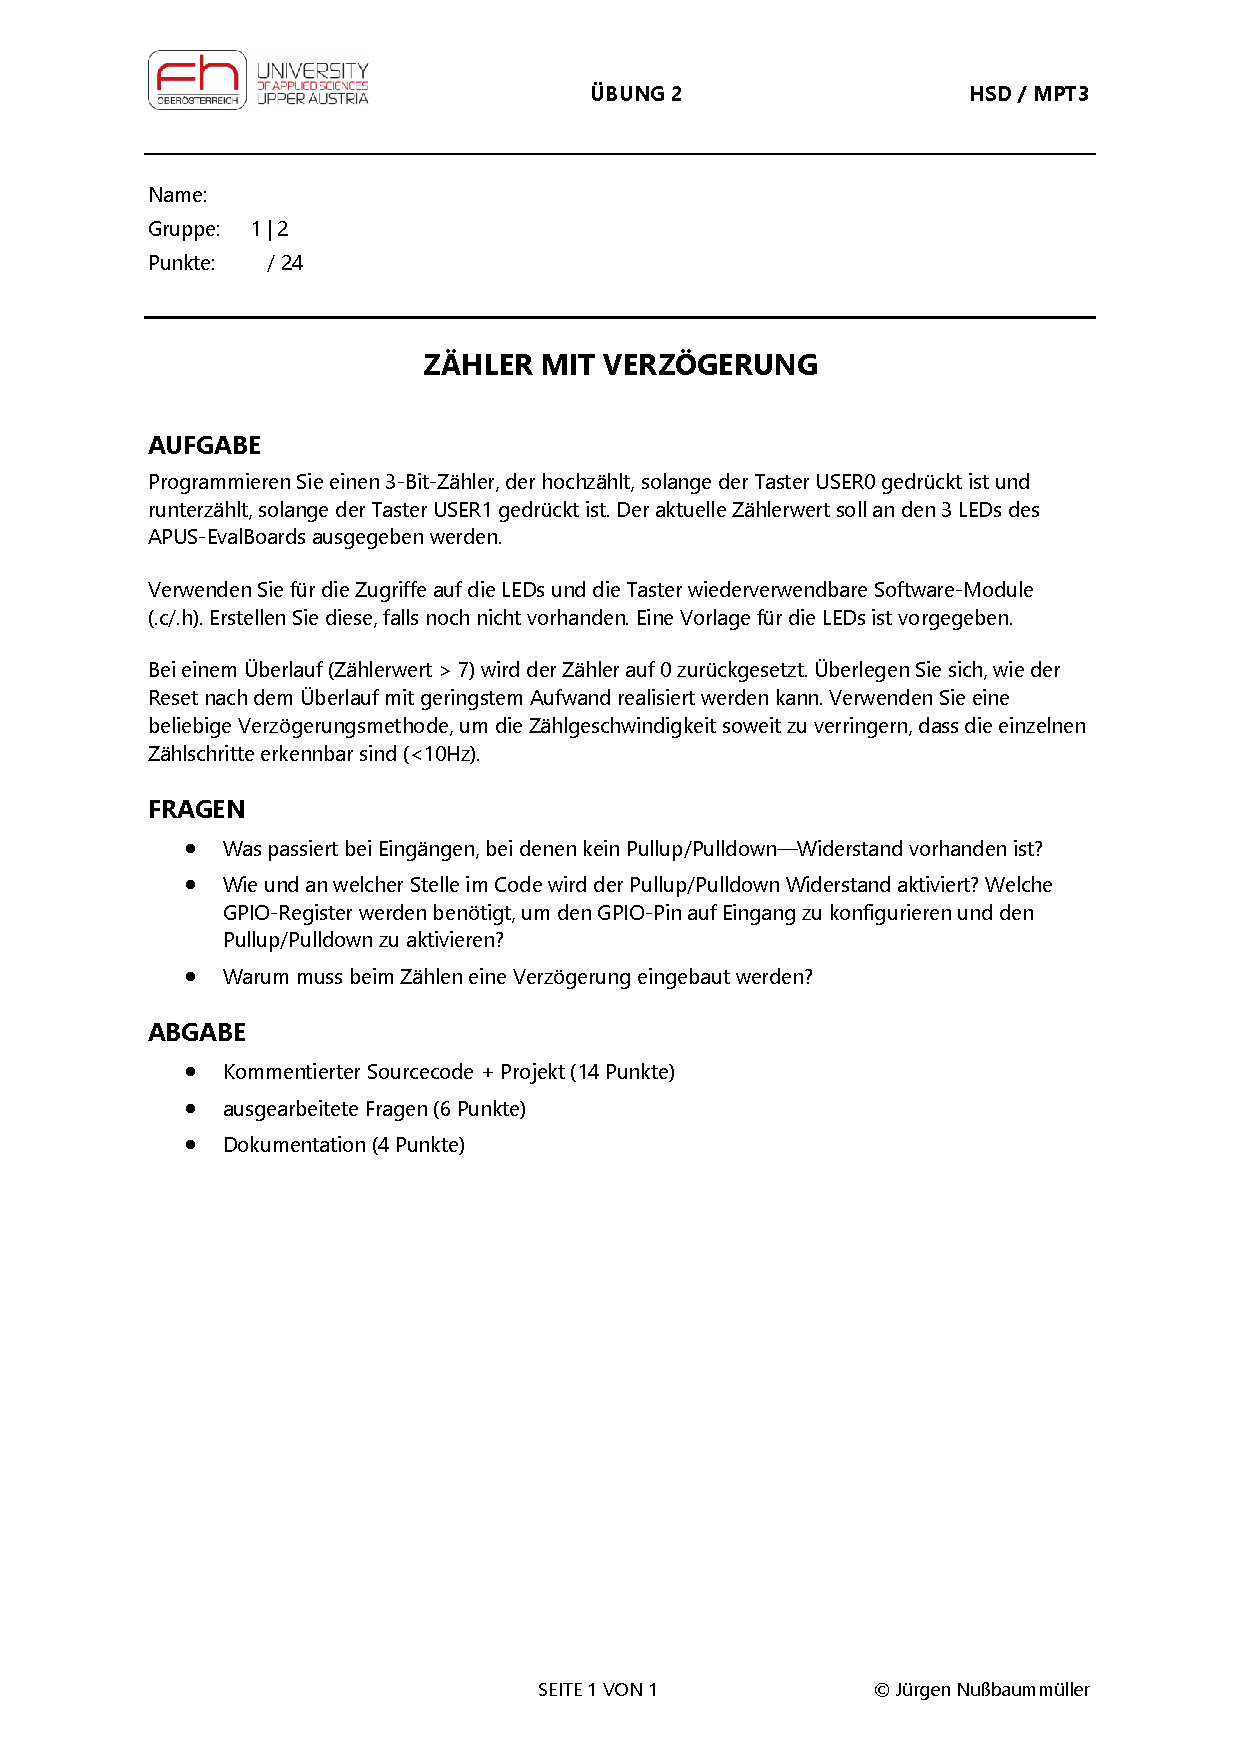
\includepdf[pages=1,pagecommand={
			\begin{textblock*}{5cm}(3.5cm, 3.1cm)
				\textbf{\name}    \textbf{\matnr}
			\end{textblock*}
		}]{./MPT3_Uebung2.pdf}

\section{Aufgabe 1:}

\subsection{Loesungsidee}


\subsection{Code}
\lstinputlisting[style=cppstyle, title=\texttt{main.c} ]{../STM32Base/projects/3_bit_Zaehler/main.c}
\lstinputlisting[style=cppstyle, title=\texttt{board\_button.h} ]{../STM32Base/system/board/board_button.h}
\lstinputlisting[style=cppstyle, title=\texttt{board\_button.c} ]{../STM32Base/system/board/board_button.c}

\subsubsection{Fragen}


\end{document}
